\chapter{Contrôles de transmission}

\section{Le protocole du bit alterné}

Nous allons ici voir un modèle de \textit{contrôle de perte de données} appelé \textit{protocole du bit alterné}.
Ce protocole a (ou plutôt avait car il a été remplacé par un protocole plus performant) lieu au sein de la couche 2 (couche lien) et permet de vérifier que les trames d'un ordinateur A sont bien reçues par un ordinateur B.\\

Le principe est très simple, il utilise les \textit{acquittements} et les \textit{flags} :  lorsque A envoie une trame, il attend un accusé de réception (acquittement, \textit{acknowledgment} en Anglais) de la part de B dans un temps imparti.\\ À ceci s'ajoute un bit de contrôle, appelé \textit{flag} en Anglais, qui alterne suivant le modèle suivant:\\

\floatpictureright{0.4}{ch-transmissions/img/bit_alterne_1}{
    \begin{itemize}
        \item 	la communication commence avec le \textit{flag} à 0, A envoie une première trame avec le \textit{flag} ;
        \item 	B reçoit la trame et accuse réception en envoyant une trame d'acquittement notée ACK. le \textit{flag} est changé à 1 ;
        \item 	A reçoit ACK avec le flag 1 et envoie donc la 2\eme trame avec ce \textit{flag} 1 ;
        \item 	et ainsi de suite : Lorsque A reçoit une trame de B, elle garde la valeur du \textit{flag} pour la prochaine trame qu'elle envoie.B, quant à lui change toujours le \textit{flag} entre le moment où il reçoit et celui ou il émet.
    \end{itemize}
}

Ce protocole permet d'éviter la perte de trames dans les cas suivants :\\

\floatpictureleft{0.4}{ch-transmissions/img/bit_alterne_2}{
    \subsection{Perte de trame du côté de A}
    A envoie la première trame et celle-ci se perd, au bout du temps imparti, ne reçoit rien.\\
    C'est ce qu'on appelle un \textit{timeout} en Anglais.\\
    A renvoie donc sa trame comme si de rien n'était.}\medskip\par

\floatpictureright{0.4}{ch-transmissions/img/bit_alterne_3}{
    \subsection{Perte de trame du côté de B} A envoie la première trame et celle-ci arrive à B, qui renvoie un ACK avec un \textit{flag} à 1, et s'attend donc à recevoir une prochaine trame avec un \textit{flag à 1}.\\
    Cette trame ACK se perd donc du point de vue de A, il y a \textit{timeout} et donc il renvoie la même trame avec le \textit{flag} à 0. B se rend compte que quelque chose ne va pas, et renvoie donc l'ACK précédent, avec son \textit{flag} à 1. La communication continue normalement.}\medskip\par

Ce protocole présente des insuffisances comme le montre l'exercice suivant

\begin{exercice}[]
    Analyse le schéma suivant et explique pourquoi il y a perte d'information.
    \begin{center}
        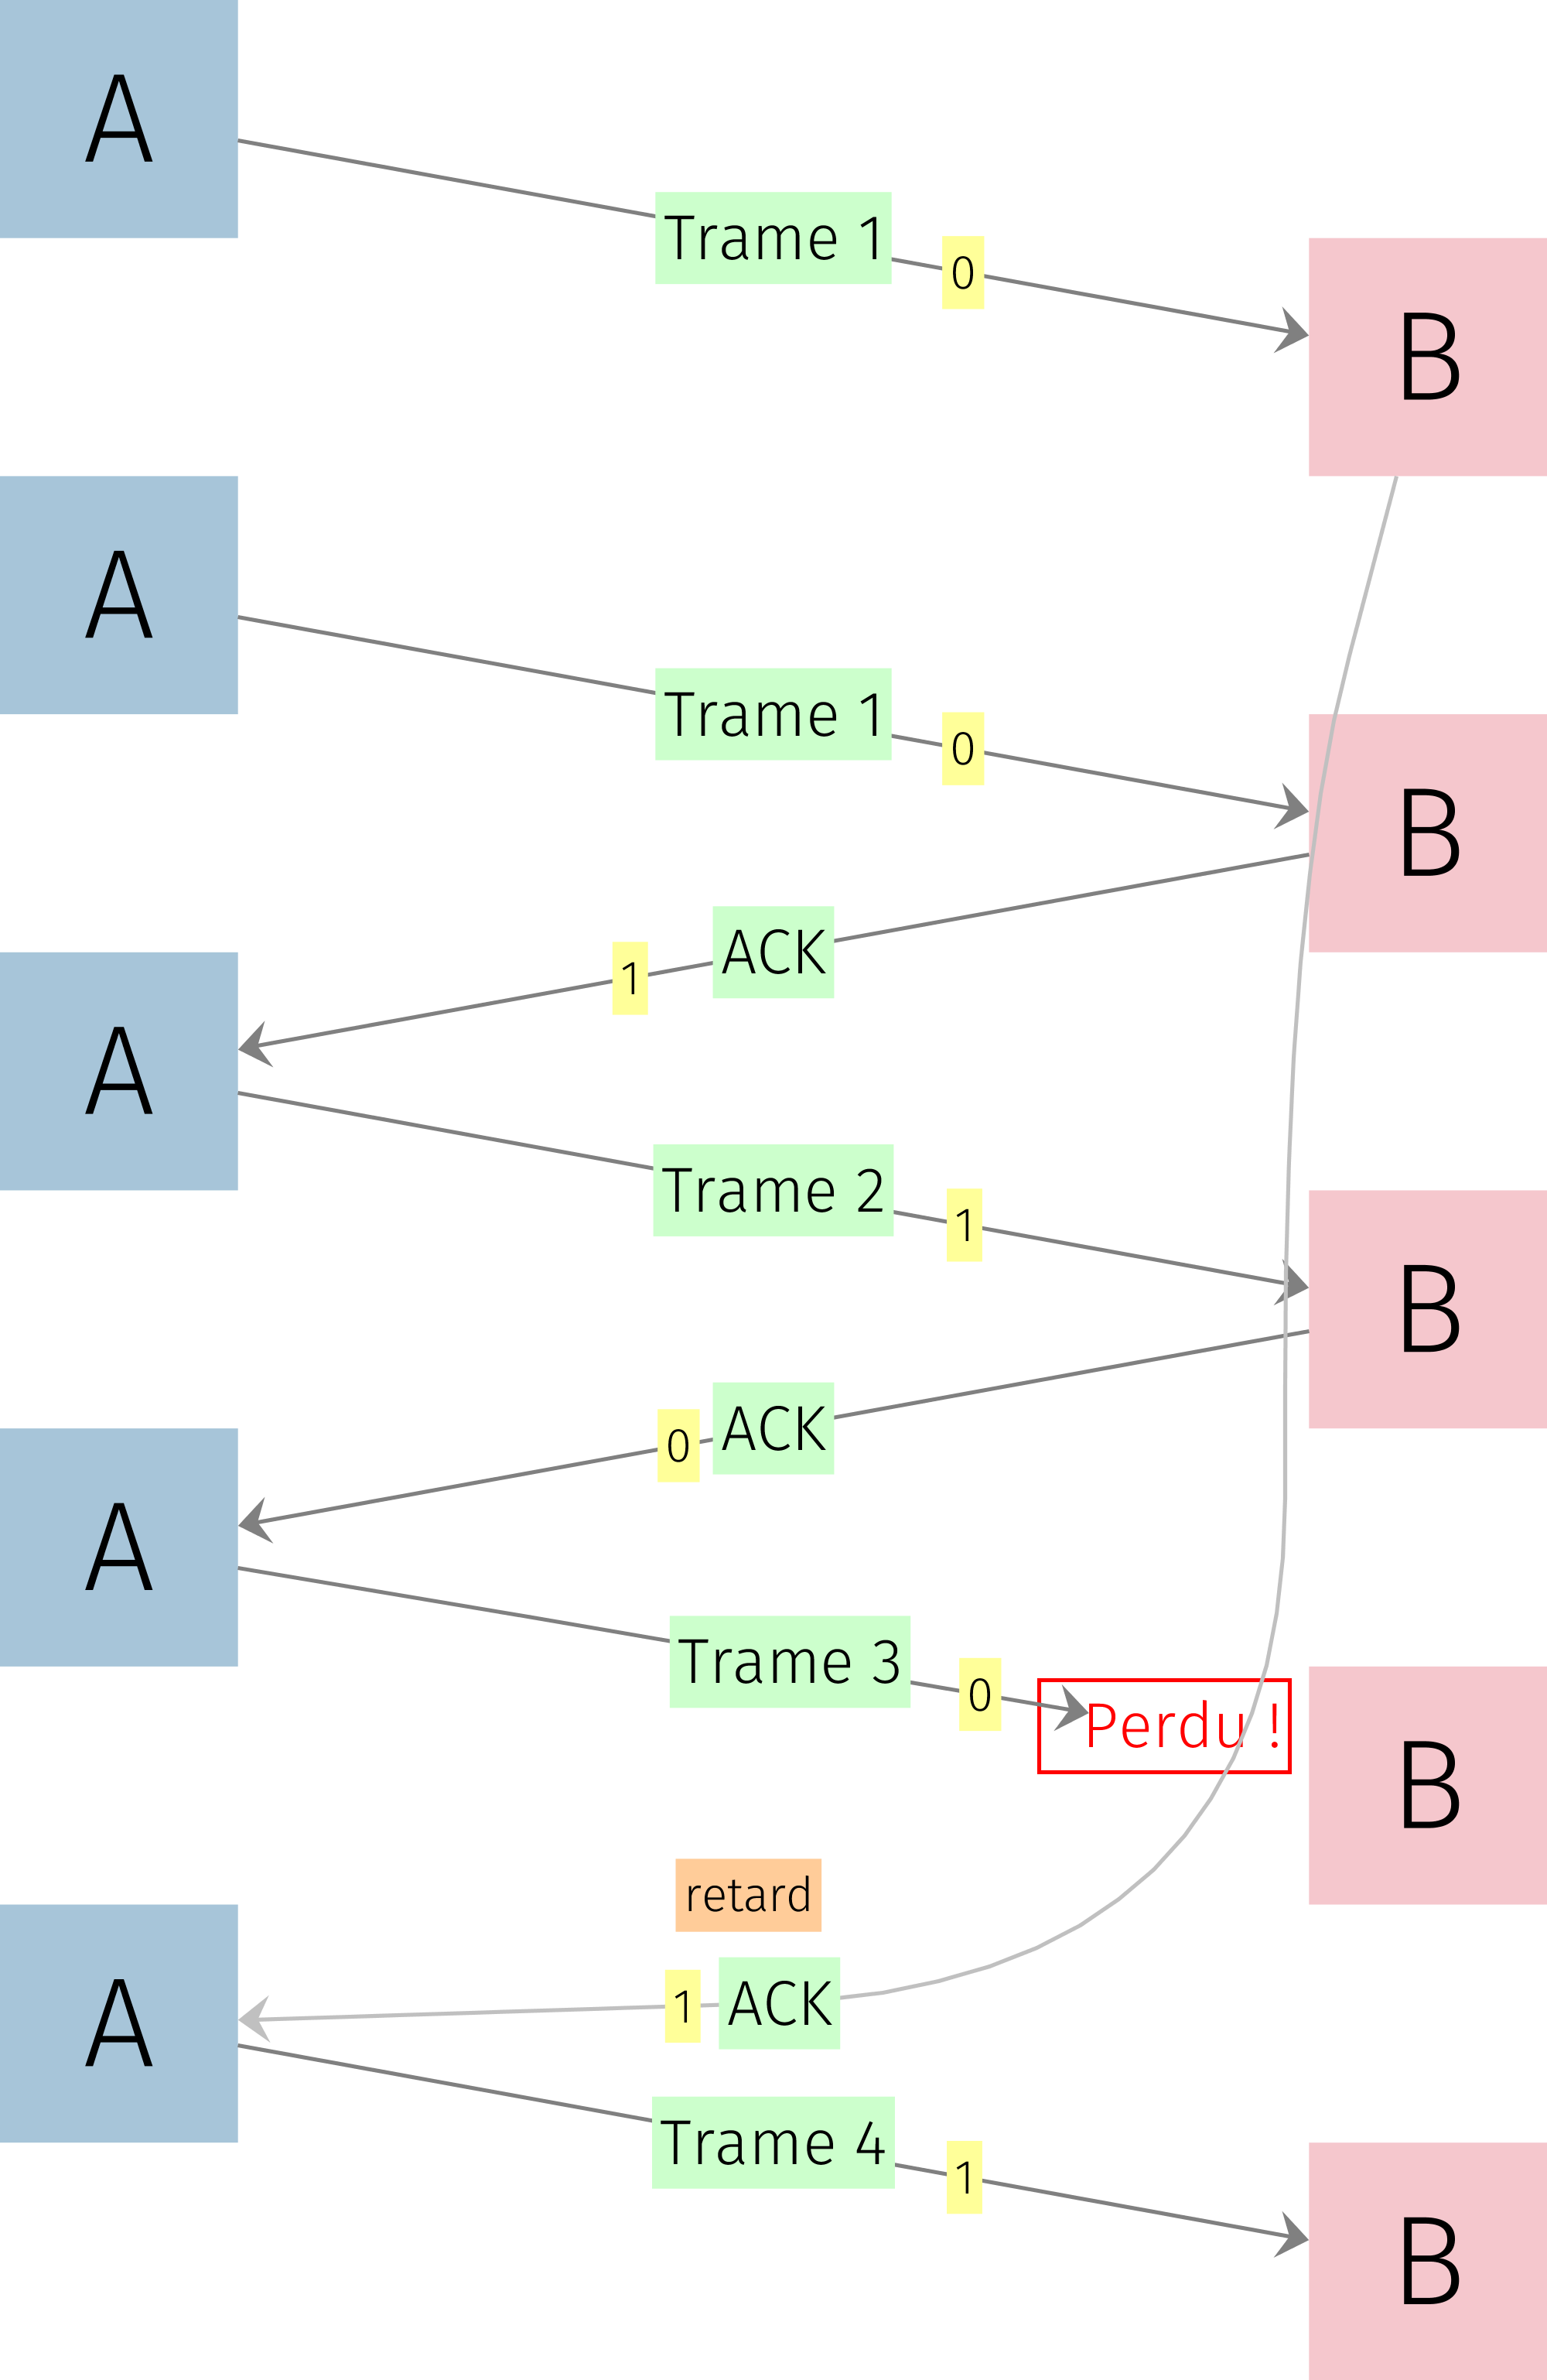
\includegraphics[width=4.2cm]{ch-transmissions/img/bit_alterne_4.png}
    \end{center}
\end{exercice}

\section{Déroulement d'une communication TCP}

On rappelle que TCP est un protocole de la couche 4 (couche transport) dont les caractéristiques principales sont les suivantes :
\begin{itemize}
    \item 	il commence par établir une connexion entre les deux machines ;
    \item 	il découpe les données en paquets ;
    \item 	il s'assure de la bonne réception des données au moyen d'\textit{accusés de réception} ;
    \item 	il met fin à la connexion.
\end{itemize}

L'exercice suivant va nous permettre d'examiner une exemple de communication TCP en détail.

\begin{exercice}[]
    Reprendre le fichier Filius de l'exercice 5 (serveur web avec DNS ) de la feuille de TP sur Filius.
    \begin{enumerate}
        \item 	En mode simulation, faire un clic droit sur 192.168.2.1 et afficher les échanges de données.
        \item	Normalement il n'y a encore eu aucune communication réseau donc la fenêtre d'échange est vide.\\
              Sur le navigateur web installé sur 192.168.2.1, entrer \texttt{monsite.com} et observer la fenêtre d'échange de données \textit{du point de vue de 192.168.2.1} :
              \begin{center}
                  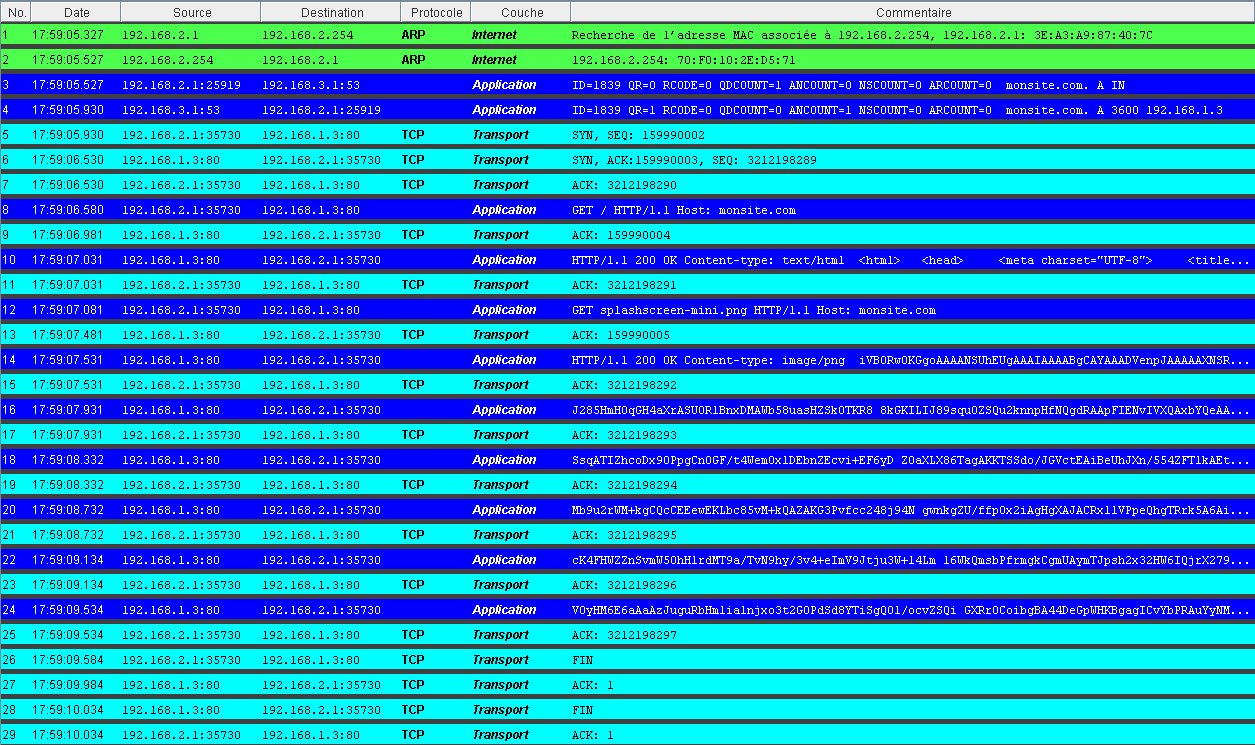
\includegraphics[width=\linewidth]{ch-transmissions/img/echange_donnees.png}
              \end{center}
              On observe 29 trames. Il est possible de cliquer sur chacune d'entre elles pour visualiser son contenu. Voici le contenu de la première :
              \begin{center}
                  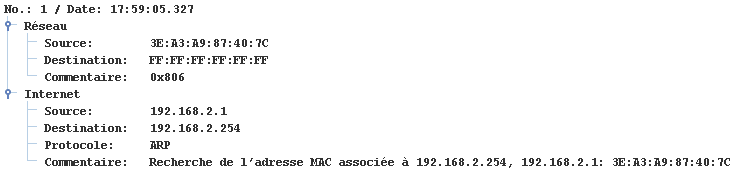
\includegraphics[width=\linewidth]{ch-transmissions/img/trame_1.png}
              \end{center}
              Il nous indique que 192.168.2.1 essaie de déterminer l'adresse MAC du routeur. En effet, 192.168.2.1 doit interroger le serveur DNS, situé en 192.168.3.1, pour obtenir l'adresse IP associée à \texttt{monsite.com}, et puisque 192.168.3.1 , n'est pas dans le même réseau que 192.168.2.1, celui-ci utilise la passerelle (le routeur).\\
              La trame suivante est la réponse ARP et la communication se poursuit.
    \end{enumerate}
    \begin{enumerate}
        \item 	Regarder la source, la destination et le contenu des trames 3 et 4. À quoi correspondent-elles ?
        \item 	On s'intéresse au début de la connexion TCP de 192.168.1.2.1 à 192.168.3.1 : ce sont les trames 5,6 et 7, qui constituent ce qu'on appelle en Anglais un \textit{Three-way handshake}. Rechercher ce terme sur Wikipédia et interpréter ensuite les 3 trames.
        \item 	Les trames 8 à 25 constituent l'échange de données en lui-même. Il y a deux grandes étapes. Lesquelles ?
        \item 	Que représentent les trames 26 à 29 ? Détailler le procédé.
    \end{enumerate}
\end{exercice}
